\section{GroupNode Class Reference}
\label{classGroupNode}\index{GroupNode@{GroupNode}}
{\tt \#include $<$GroupNode.h$>$}

Inheritance diagram for GroupNode:\nopagebreak
\begin{figure}[H]
\begin{center}
\leavevmode
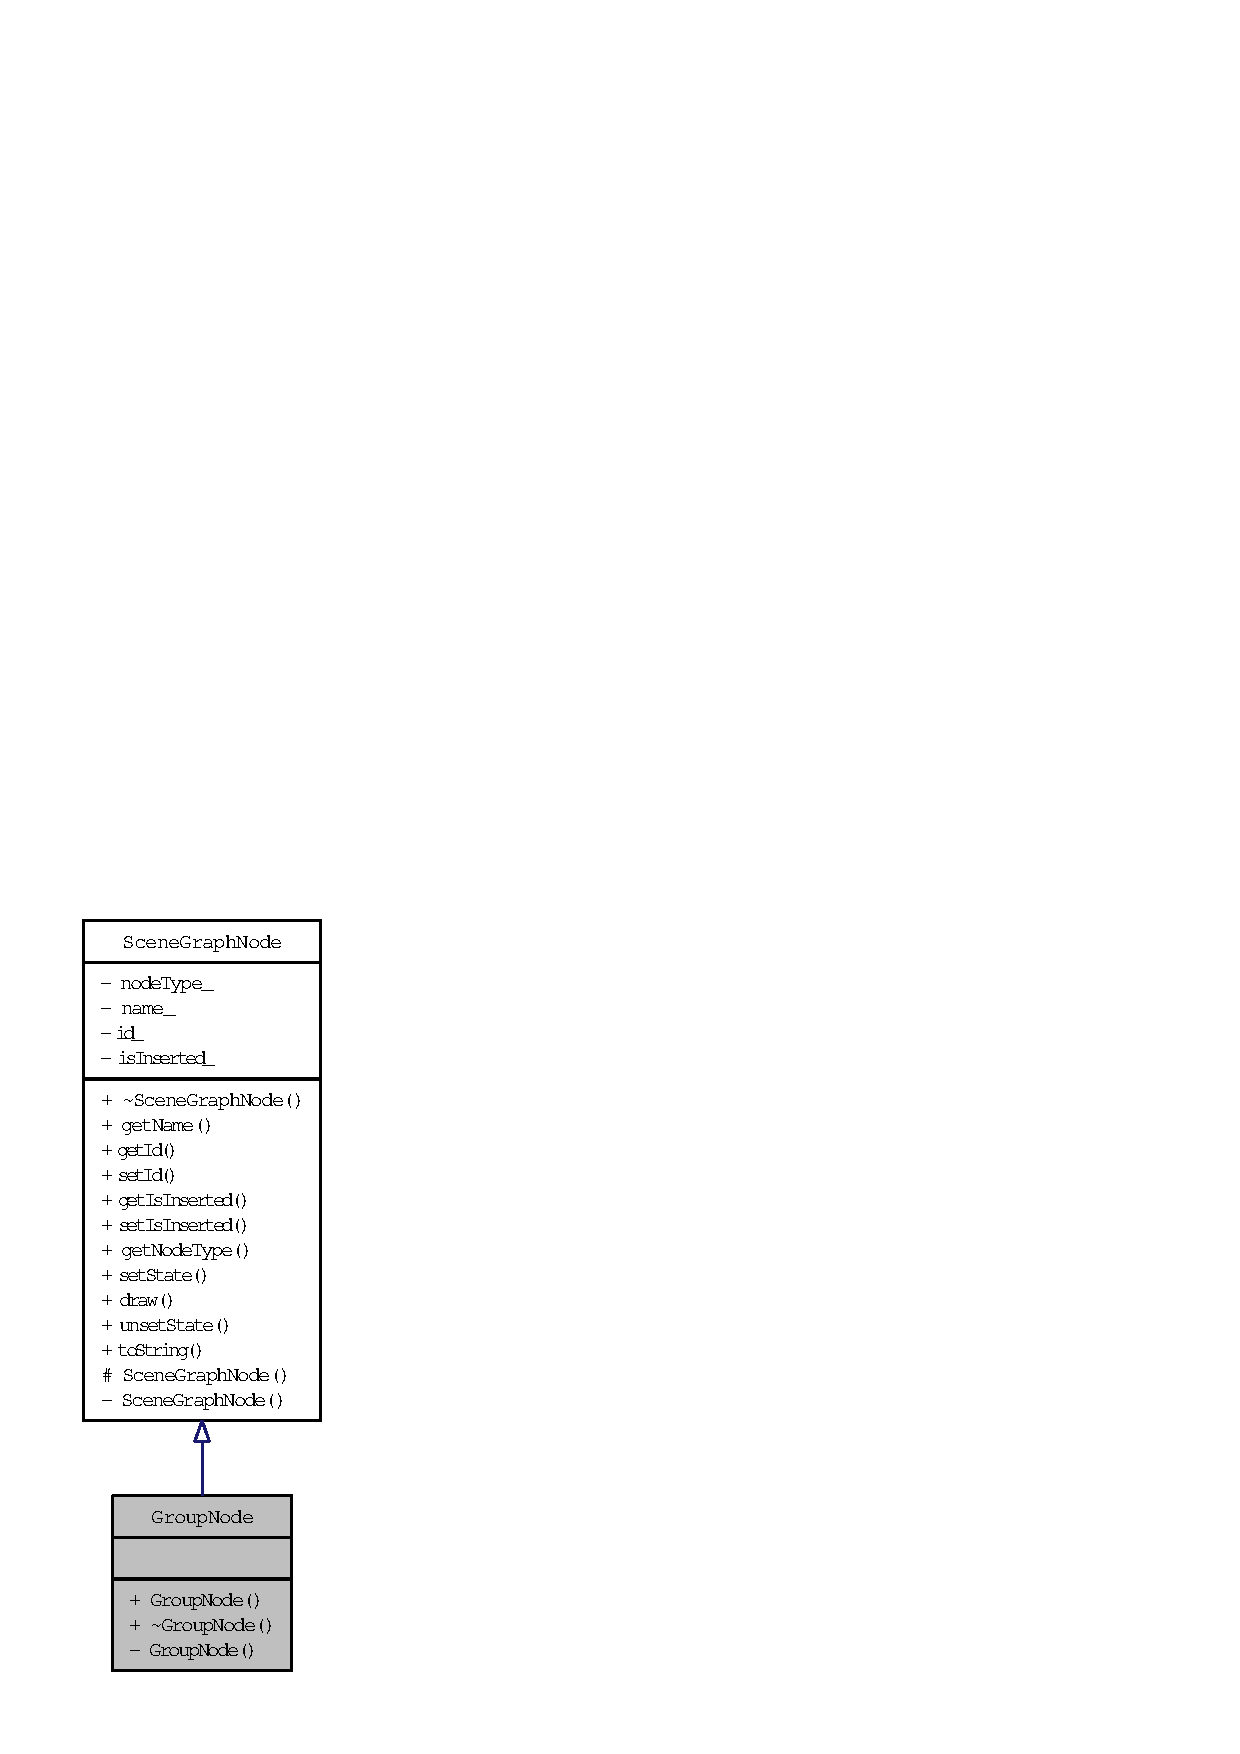
\includegraphics[height=400pt]{classGroupNode__inherit__graph}
\end{center}
\end{figure}
Collaboration diagram for GroupNode:\nopagebreak
\begin{figure}[H]
\begin{center}
\leavevmode
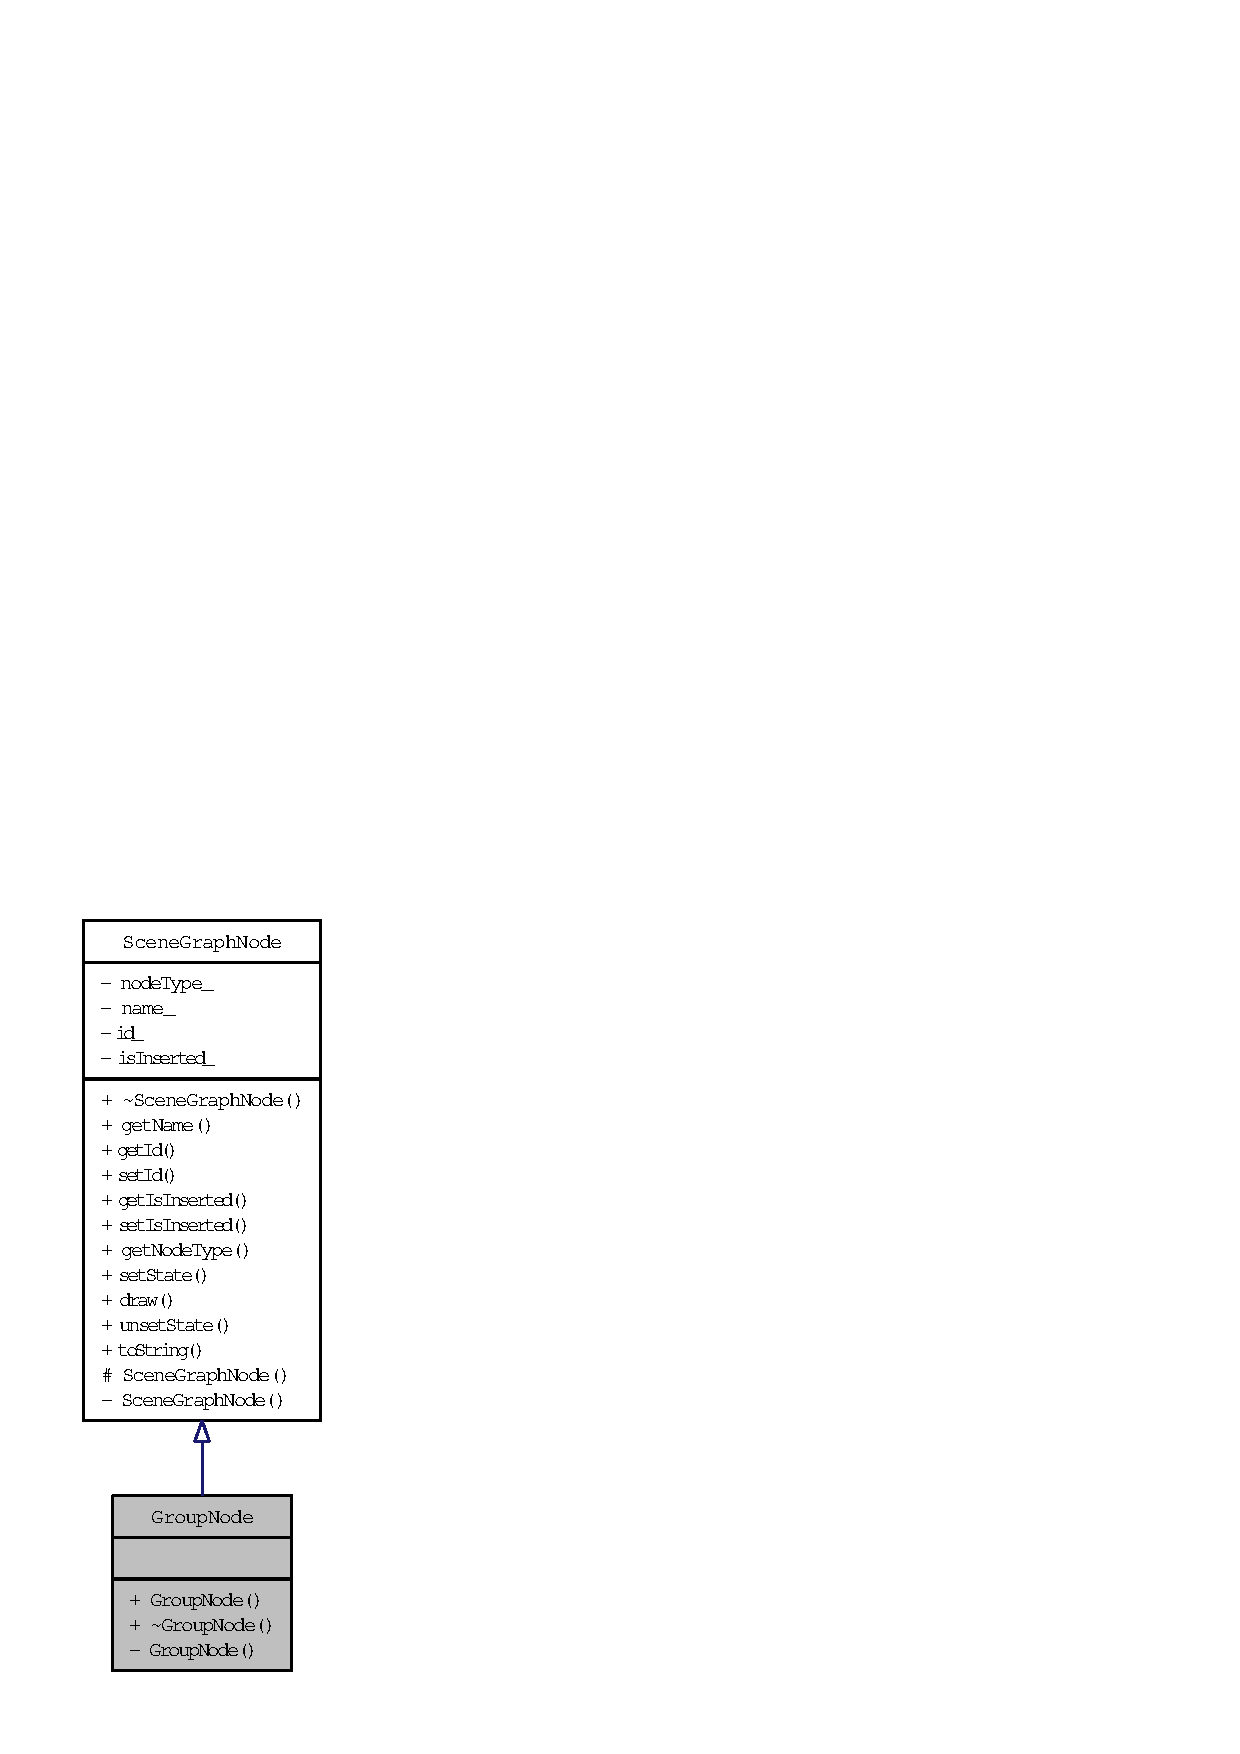
\includegraphics[height=400pt]{classGroupNode__coll__graph}
\end{center}
\end{figure}


\subsection{Detailed Description}
This is a simple grouping node that is used to gather nodes together it implementation of setState and draw are the default empty it is node thats name captures the semantics of grouping other nodes. 

Definition at line 18 of file GroupNode.h.\subsection*{Public Member Functions}
\begin{CompactItemize}
\item 
{\bf GroupNode} (std::string name)
\begin{CompactList}\small\item\em \begin{Desc}
\item[Parameters:]
\begin{description}
\item[{\em name}]the descriptive name of the node constructor \end{description}
\end{Desc}
\item\end{CompactList}\item 
virtual {\bf $\sim$GroupNode} (void)
\begin{CompactList}\small\item\em destructor \item\end{CompactList}\end{CompactItemize}


\subsection{Constructor \& Destructor Documentation}
\index{GroupNode@{GroupNode}!GroupNode@{GroupNode}}
\index{GroupNode@{GroupNode}!GroupNode@{GroupNode}}
\subsubsection{\setlength{\rightskip}{0pt plus 5cm}GroupNode::GroupNode (std::string {\em name})}\label{classGroupNode_a692e635b5fe5ddb4ecad4aecae7d267}


\begin{Desc}
\item[Parameters:]
\begin{description}
\item[{\em name}]the descriptive name of the node constructor \end{description}
\end{Desc}




Definition at line 4 of file GroupNode.cpp.\index{GroupNode@{GroupNode}!$\sim$GroupNode@{$\sim$GroupNode}}
\index{$\sim$GroupNode@{$\sim$GroupNode}!GroupNode@{GroupNode}}
\subsubsection{\setlength{\rightskip}{0pt plus 5cm}GroupNode::$\sim$GroupNode (void)\hspace{0.3cm}{\tt  [virtual]}}\label{classGroupNode_76112483fe680b62637195541a017e75}


destructor 



Definition at line 8 of file GroupNode.cpp.

The documentation for this class was generated from the following files:\begin{CompactItemize}
\item 
{\bf GroupNode.h}\item 
{\bf GroupNode.cpp}\end{CompactItemize}
